\documentclass{scrartcl}

\usepackage[utf8]{inputenc}
\usepackage{graphicx}
\usepackage[noabbrev]{cleveref}

\title{Project Report\\
Group gingerbread}

\subtitle{Java and C\# in depth, Spring 2014}

\author{Patrick Lüthi\\
Simon Marti\\
Nadja Müller}

\begin{document}

\maketitle

\section{Introduction}
This document describes the design and implementation of the {\it Personal
Virtual File System} of group gingerbread. The project is part of the course
{\it Java and C\#} in depth at ETH Zurich. The following sections describe each
project phase, listing the requirements that were implemented and the design decisions taken.
The last section describes a use case of using the {\it Personal Virtual File
System.}

\section{VFS Core}
The VFS core provides an API to facilitate creating, modifying and deleting
virtual disks, importing and exporting files from the host file system and
manipulating files on virtual disks.

\subsection{Requirements}

	\begin{description}
	\item[Single-File Storage] \ \\
		The virtual disk is stored in a single file in the working directory in
		the host file system.
	\item[Disk Creation] \ \\
		Disks can be created with a specified maximum size at a specified location.
	\item[Disk Disposal] \ \\
		Entire disks can be deleted with {\tt VirtualDisk.Delete()}.
	\item[Directory Manipulation] \ \\
		Directories can be created, deleted, renamed, copied and moved through {\tt
		VirtualDirectory}'s exposed API.
	\item[Navigation] \ \\
		Files and directories can be accessed using relative file paths from
		any directory ({\tt VirtualDirectory.GetRelativeItem()}).
	\item[File Import and Export] \ \\
		Files can be imported from and exported to the host file system using the
		respective methods of {\tt VirtualDirectory} and {\tt VirtualFile}.
	\item[Usage Information] \ \\
		The {\tt VirtualDisk} exposes the number of free files ({\tt FreeFiles}) and
		bytes ({\tt FreeSpace}) as well as the total available space ({\tt
		TotalSpace}) as public properties.
	\item[Elastic Disk] \ \\
		The virtual disk dynamically grows when new files are added.
	\item[Large Data] \ \\
		Files are not completely loaded into memory during import and export, allowing
		very large files to be handled.
	\end{description}

\subsection{Design}
The implementation of the VFS core is split into two main parts. One part being
the container file framework and the other the virtual file system implementation itself.


\subsubsection{The container file framework}
We decided to design an abstracted file system that only uses low level file descriptions and
a single layer file hierarchy first. As this abstracted file system is stored in
a single file on the host file system and this file acts as a container for all
the files it might contain it was called a container file. The container file
framework would provide all features associated to a container file. The
framework provides a simple interface for creating and deleting files as well as
reading and writing to a file in a uniform way. The interface hides the
underlying representation of the data associated to the file thereby increasing modularity.

\paragraph{The container file structure} \ \\
We decided to implement our system closely related to the unix file system.
The file is split into a sequence of equally sized blocks. The first block is
the super block containing information about the container file like maximum
size or the number of remaining free index nodes. It is followed by several
blocks which contain index nodes. The remaining blocks are dynamically used to
either store pointers to additional file blocks, free data blocks lists, or file
data directly.

\paragraph{Index node structure} \ \\
Index nodes are currently 32 bytes in size consisting of one unsigned integer
denoting the number of data blocks associated with this index node, 4 direct
pointers to data blocks, 1 indirect pointer, 1 double indirect pointer and one
triple indirect pointer. Aside from the number of different pointer types it
works in a similar way to the index node in the unix file system:
The direct pointers point to data blocks directly. The indirect pointer points
to a block of pointers to data blocks. The double indirect pointer points to a
block of pointers that point to a block of pointers that point to a data block.

\paragraph{Free blocks management} \ \\
The superblock contains a stack of free blocks.
If the stack has more than one element the top of the stack is removed and
returned as a free block.
Once the stack only has one element left and the element is not zero then this
means that this last block contains further free blocks. The superblock's free
blocks stack is refreshed using the content of said block and the block itself
is afterwards returned as a free block.
If the stack only contains the element zero that means there are currently no
free blocks to be reallocated. In this case the system may allocate a
completely new block at the end of the container file as long as the maximum
capacity is not yet reached.
The freeing process just works in reverse logic.

\paragraph{Caching} \ \\
In order to reduce the number of read and write operations to the disk we
implemented a component called block manager which caches a certain amount of
blocks. It uses a least recently used eviction strategy and only writes back
blocks that were marked as being potentially modified.

\paragraph{File stream} \ \\
Objects of this class are used to access or modify data belonging to a certain
file using the same interface as if the client was writing to an actual file in
the host file system. It internally handles the segmentation of the data
associated to the file.


\subsubsection{The virtual file system} \ \\
The virtual file system part of the VFS core implements the necessary higher
level logic (file names, directory hierarchies, importing/exporting) using the
container file framework.

\paragraph{Virtual disk} \ \\
The main access points are virtual disk objects containing virtual items like directories and files.
Virtual files and directories are managed as files in a container file and
therefore the virtual file system can manage the representation of virtual
items as if they were stored in a separate file with continuous memory.
A virtual disk object defines a designated root directory which is the top most
parent of every file stored in the VFS.
Operations are then performed on virtual disk or virtual item objects directly.
Navigation happens implicitly by retrieving child items given a parent item.
Additionally information about the disk state (free/occupied space) can be
retrieved using corresponding properties of a virtual disk item.

\paragraph{Virtual directory} \ \\
Virtual directories provide operations on the logical directory they represent. Currently the contents of a directory are stored as a sequential list of child item entries.

\paragraph{The public interface} \ \\
\Cref{fig:coreapi} describes the public API of the VFS core.
\begin{figure}[h]
    \centering
        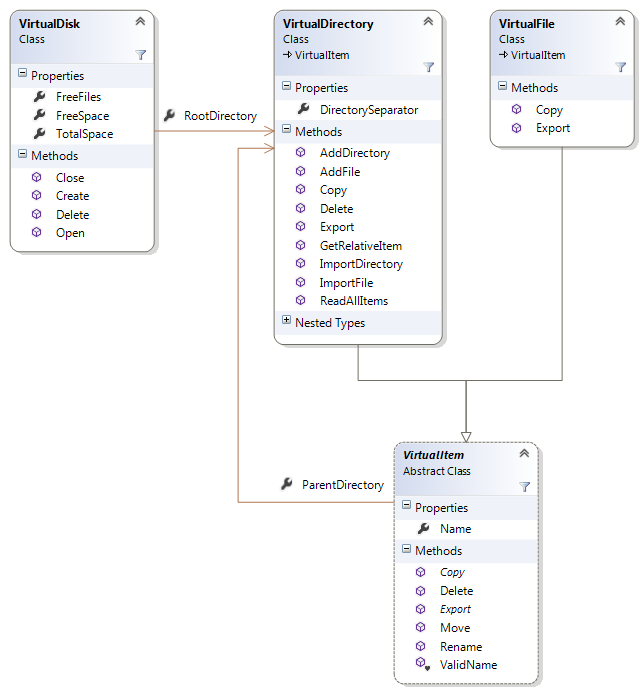
\includegraphics[width=0.8\textwidth]{figures/PublicInterfaceVFSCore}
        \caption{Public interface of the VFS core.}
        \label{fig:coreapi}
\end{figure}

\end{document}
